\documentclass[tikz,crop]{standalone}

\usepackage[T1]{fontenc}
\usepackage[tt=false,type1=true]{libertine}
\usepackage[varqu]{zi4}
\usepackage{newtxmath}
\usepackage[dvipsnames]{xcolor}
\usepackage{tikz}
\usepackage{marvosym}
\usepackage[marvosym]{tikzsymbols}
\usetikzlibrary{arrows, matrix, arrows.meta, shapes, shapes.arrows, shapes.multipart, shapes.symbols, fadings, fit, positioning, decorations.pathreplacing, angles, quotes}

\begin{document}

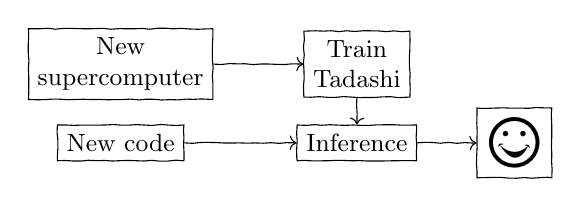
\begin{tikzpicture}[
  decoration={random steps,segment length=1mm,amplitude=0.2pt},
  every node/.style={decorate, draw}, align=center, font=\small,
  every edge/.style={decorate, draw, ->},
]
\node (new) {New\\supercomputer};
\node [right of=new, node distance=3cm] (train) {Train\\Tadashi};
\node [below of=new] (newcode) {New code};
\node [below of=train] (infer) {Inference};
\node [right of=infer, node distance=2cm] (done) {\Huge \Smiley};
\path
(new) edge (train)
(newcode) edge (infer)
(train) edge (infer)
(infer) edge (done);
\end{tikzpicture}
\end{document}
